\documentclass[12pt]{report}

\usepackage[english]{babel}
\usepackage[utf8x]{inputenc}
\usepackage{amsmath}
\usepackage{graphicx}
\usepackage{multirow}
\usepackage[hypcap]{caption}
\usepackage{setspace} 
\usepackage{float}

\title{Lab 10: Fractography and Fracture Toughness Testing}
\author{Zachary Tschirhart \\
	\small \\
        \small EID: zst75 \\
	\small Department of Aerospace Engineering and Engineering Mechanics \\
	\small \textbf{ASE 324L (Mon 2:00-5:00)} \\
	\small Unique: 13740}

\date{April 15, 2014}


\begin{document}
\maketitle

\begin{abstract}
Aluminum alloy specimens with varying thickness had tensile loads applied until the specimen fractured and eventually failed. Before the experiment took place, each specimen was initially loaded until a fatigue crack formed. While the specimen were placed under the tensile load, time and load were recorded. After the specimen failed, it was inspected to measure crack length and any other properties that needed to be recorded. Based on the results, as the thickness of a specimen decreases, the fracture toughness increases.

\end{abstract}


\tableofcontents
\pagebreak

\setcounter{secnumdepth}{0}

\section{Introduction}
\doublespacing
Knowing how and why structures fail is an integral part of engineering any structure, especially when lives are at stake. For the purpose of aerospace applications, cracks forming in the structure need to be understood and what margin of safety is required. Aluminum alloy is a common material used in aerospace applications, so studying this material can be directly related to the field. 

\section{Experimental and Data Reduction Procedures}
\subsection{Procedure}
Three specimen were tested with varying thickness, one at 0.5 inches, another at 0.25 inches, and the last at 0.125 inches. Before the specimen were tested in the lab, initial cracks were produced by cyclic loading. During the lab, the specimen were put under a tensile load until failure occurred while recording the load at specific times. Each specimen was loaded using a constant cross-head displacement rate of 0.06 inches per minute. After the specimen was removed from the testing apparatus, the crack length and width was recorded.

\subsection{Data Reduction}
In order to calculated the fracture toughness for each specimen, the following equation was used:

\begin{equation}
\begin{split}
  K_c = \frac{P_{max}}{bW^{1/2}} * (29.6x^{1/2} - 185.5x^{3/2} + 655.7x^{5/2} - 1017x^{7/2} + 639x^{9/2})
  \label{equation:equation1}
\end{split}
\end{equation}
\\
where \(K_c\) is the fracture toughness, b is the specimen thickness, W is the specimen width, \(P_{max}\), and x is the crack length divided by specimen width.


In order to determine if the plane strain fracture toughness (Kic) can be used, the following equation needs to be used:

\begin{equation}
\begin{split}
  a,b >= 2.5(\frac{K_c}{\sigma_{y}})^2
  \label{equation:equation2}
\end{split}
\end{equation}
\\
Where a is the crack length and \(\sigma_y\) is the yield stress. Using this equation will help determine if the fracture toughness satisfies the condition known as the plane-strain fracture toughness.


To measure compliance in the linear region for each specimen, a simple equation is used to calculate the value:

\begin{equation}
\begin{split}
  C = \frac{\Delta}{P}
  \label{equation:equation3}
\end{split}
\end{equation}
\\

Where C is the compliance value, \(\Delta\) is the change in cross-head displacement, and P is the load value. 

\section{Results and Discussion}
\doublespacing
The purpose of this lab was to determine the fracture toughness and compliance of each specimen tested. In the following figures, the values of fracture toughness were plotted against the crack lengths for different specimen. 

\begin{figure}[H]
	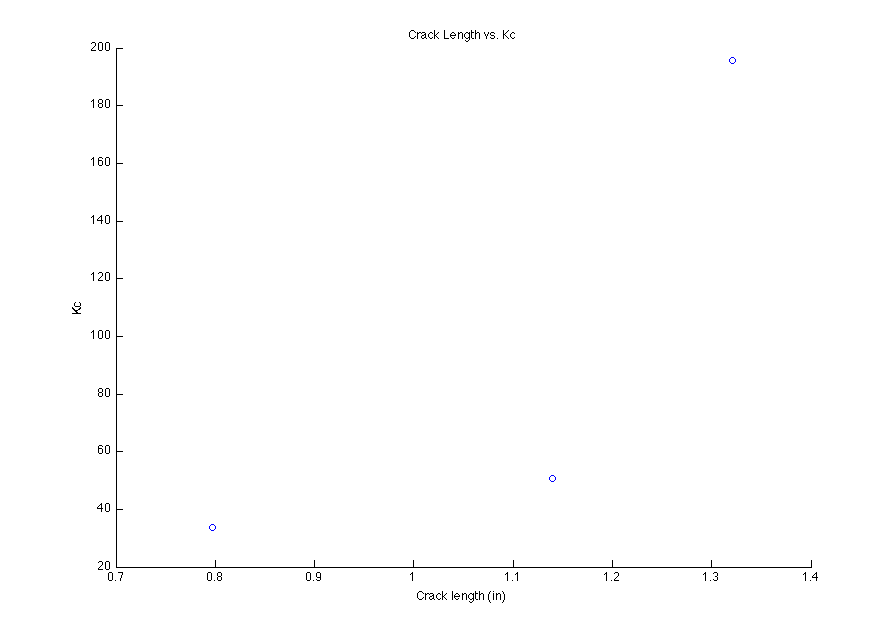
\includegraphics[width=1\textwidth]{crack_vs_kc.png}
	\caption{Fracture Toughness versus Crack Length}
	\label{fig:Figure1}
\end{figure}
\\
\\

Now averaging the fracture toughness between all specimen tested in the labs, Figure 2 shows that as thickness increases, the average fracture toughness decreases.

\begin{figure}[H]
	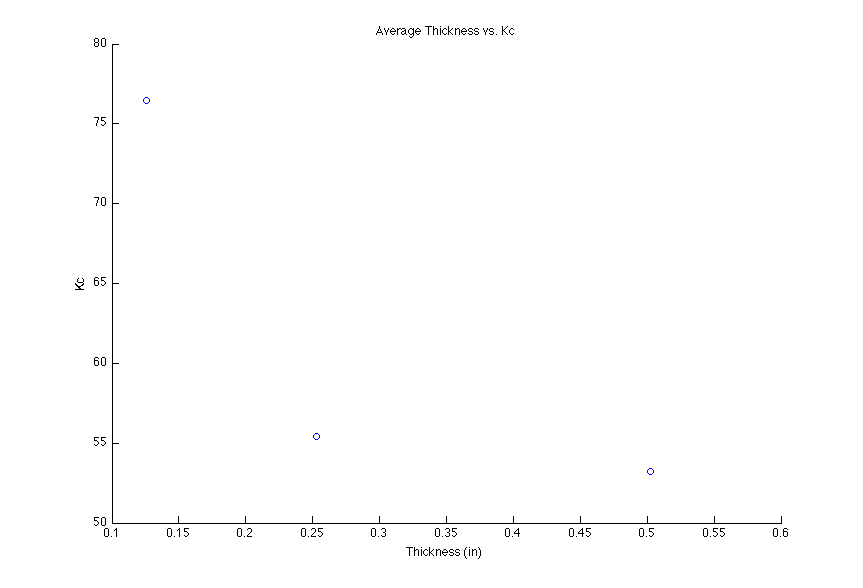
\includegraphics[width=1\textwidth]{avgt_vs_kc.png}
	\caption{Average Fracture Toughness versus Thickness}
	\label{fig:Figure2}
\end{figure}
\\
\\



\begin{figure}[H]
    \singlespacing
    \begin{tabular}{| l | l | l | l | l |}
    \hline
    Specimen Thickness (in) & Width (in) & Crack Length (in) & Kc (ksi) & Compliance \\ \hline
    0.50233 & 2.03692 & 1.26067 & 53.21273 & 76.70615\\ \hline
    0.25252 & 2.04142 & 0.86001 & 55.41589 & 65.13411\\ \hline
    0.12567 & 2.01167 & 1.10950 & 76.48799 & 26.37277\\ \hline
    \end{tabular}
    \caption{Average values of all eighteen specimen}
\end{figure}
\doublespacing

\section{Fractographs Observation}


\section{Conclusion}
\doublespacing



\begin{thebibliography}{0}
\bibitem{notes} {\em ASE 324L Lab manual : The University of Texas at Austin Department of Aerospace Engineering}  2014.
\bibitem{notes} {\em ASE 324L Lecture 19 : The University of Texas at Austin Department of Aerospace Engineering}  2014.
\bibitem{notes} {\em ASE 324L Lecture 20 : The University of Texas at Austin Department of Aerospace Engineering}  2014.
\end{thebibliography}
\addcontentsline{toc}{section}{Bibliography}


\end{document}
